\documentclass[a4paper,12pt]{report}
\usepackage[dvipsnames]{xcolor}
\usepackage[utf8]{inputenc} % style d'écriture
\usepackage[T1]{fontenc}      % package
\usepackage[francais]{babel}  % package pour langue française
\usepackage[a4paper]{geometry} % definition des marges
\usepackage[pdftex]{graphicx} % definition d'image
\usepackage{fancyhdr} % haut de page
\usepackage{float}
\usepackage{tcolorbox,listings}
\usepackage{caption}
\addtocounter{tocdepth}{3}
\setcounter{secnumdepth}{3}
\usepackage{color}


\lstset{
  aboveskip=5mm,
  belowskip=-2mm,
  basicstyle=\footnotesize,
  breakatwhitespace=false,
  breaklines=true,
  captionpos=b,
  commentstyle=\color{red},
  deletekeywords={...},
  escapeinside={\%*}{*)},
  extendedchars=true,
  framexleftmargin=16pt,
  framextopmargin=3pt,
  framexbottommargin=6pt,
  frame=tb,
  keepspaces=true,
  keywordstyle=\color{blue},
  language=VHDL,
  literate=
  {²}{{\textsuperscript{2}}}1
  {⁴}{{\textsuperscript{4}}}1
  {⁶}{{\textsuperscript{6}}}1
  {⁸}{{\textsuperscript{8}}}1
  {€}{{\euro{}}}1
  {é}{{\'e}}1
  {è}{{\`{e}}}1
  {ê}{{\^{e}}}1
  {ë}{{\"{e}}}1
  {É}{{\'{E}}}1
  {Ê}{{\^{E}}}1
  {û}{{\^{u}}}1
  {ù}{{\`{u}}}1
  {â}{{\^{a}}}1
  {à}{{\`{a}}}1
  {á}{{\'{a}}}1
  {ã}{{\~{a}}}1
  {Á}{{\'{A}}}1
  {Â}{{\^{A}}}1
  {Ã}{{\~{A}}}1
  {ç}{{\c{c}}}1
  {Ç}{{\c{C}}}1
  {õ}{{\~{o}}}1
  {ó}{{\'{o}}}1
  {ô}{{\^{o}}}1
  {Õ}{{\~{O}}}1
  {Ó}{{\'{O}}}1
  {Ô}{{\^{O}}}1
  {î}{{\^{i}}}1
  {Î}{{\^{I}}}1
  {í}{{\'{i}}}1
  {Í}{{\~{Í}}}1,
  morekeywords={*,...},
  numbers=left,
  numbersep=10pt,
  numberstyle=\tiny\color{black},
  rulecolor=\color{black},
  showspaces=false,
  showstringspaces=false,
  showtabs=false,
  stepnumber=1,
  stringstyle=\color{gray},
  tabsize=4,
  title=\lstname,
}

%\captionsetup[figure]{labelformat=empty}
\renewcommand{\thesection}{\Roman{section}}

\begin{document}
   \begin{titlepage}
    
    \newcommand{\HRule}{\rule{\linewidth}{0.5mm}} % Defines a new command for the horizontal lines, change thickness here
    
    \center % Center everything on the page
     
    %----------------------------------------------------------------------------------------
    %	HEADING SECTIONS
    %----------------------------------------------------------------------------------------
    
    \textsc{\LARGE Université de Bretagne Occidentale}\\[1.5cm] % Name of your university/college
		\textsc{\Large Master 2 Informatique}\\[0.5cm] % Major heading such as course name
		\textsc{\Large Département Informatique}\\[1.5cm] % Major heading such as course name
		{\large 2020/2021}\\[1.5cm] % Date, change the \today to a set date if you want to be precise
		
    \textsc{\large Mobiles et Objets Connectés}\\[1cm] % Minor heading such as course title
    
    %----------------------------------------------------------------------------------------
    %	TITLE SECTION
    %----------------------------------------------------------------------------------------
    
   \HRule \\[0.4cm]
    { \huge \bfseries La Matrice Connecté}\\[0.2cm] % Title of your document
    \HRule \\[1cm]
     
    %----------------------------------------------------------------------------------------
    %	AUTHOR SECTION
    %----------------------------------------------------------------------------------------
    
    \begin{minipage}{0.48\textwidth}
			\begin{flushleft} \large
				\emph{Auteur:}\\
					Maureen \textsc{PERON} % Your name
			\end{flushleft}
    \end{minipage}
		~
		\begin{minipage}{0.48\textwidth}
			\begin{flushright} \large
				\emph{Auteur:}\\
					Timothé \textsc{LANNUZEL} % Your name
			\end{flushright}
    \end{minipage}\\[0.5cm]
		
		\begin{minipage}{0.48\textwidth}
			\begin{center} \large
				\emph{Auteur:}\\
					William \textsc{PENSEC} % Your name
			\end{center}
    \end{minipage}\\[1.5cm]
    
    %----------------------------------------------------------------------------------------
    %	DATE SECTION
    %----------------------------------------------------------------------------------------
    
    {\today}\\[1.5cm] % Date, change the \today to a set date if you want to be precise
    
    %----------------------------------------------------------------------------------------
    %	LOGO SECTION
    %----------------------------------------------------------------------------------------
    
		\begin{minipage}{0.48\textwidth}
			\begin{flushleft} \large
				
\includegraphics[scale=0.8]{ubo_sc.png} % Include a department/university logo - this will require the graphicx package
			\end{flushleft}
    \end{minipage}
		~
    \begin{minipage}{0.48\textwidth}
			\begin{flushright} \large
				
\includegraphics[scale=0.5]{ubo.png} % Include a department/university logo - this will require the graphicx package
			\end{flushright}
    \end{minipage}
    
    %----------------------------------------------------------------------------------------
    
    \vfill % Fill the rest of the page with whitespace
    
    \end{titlepage}
		
	\pagestyle{fancy}
		\lhead{Rapport Projet MOC}
		\chead{}
		\rhead{Matrice Connectée}
		\lfoot{}
		\cfoot{\thepage}
		\rfoot{}
		
	\newpage\renewcommand{\contentsname}{Sommaire}
	\tableofcontents

	\newpage
	\section{Introduction}
		\paragraph*{}
		Ce rapport décrit le travail effectué pour le projet avec en détail les architectures choisies.
		
		Le projet consistait à la réalisation d’un jeu constitué d’un point se trouvant dans une grille et qui peut être déplacé via téléphones ou des commandes à distances.
Le code réalisé peut etre retouvé sur Github: https://github.com/WilliamPsc/ MatriceConnectee\_IoT
	
	\section{Travail effectué}
		\subsection{Épisode 1}
			\paragraph*{}
			
			\begin{figure}[H]
				\centering
					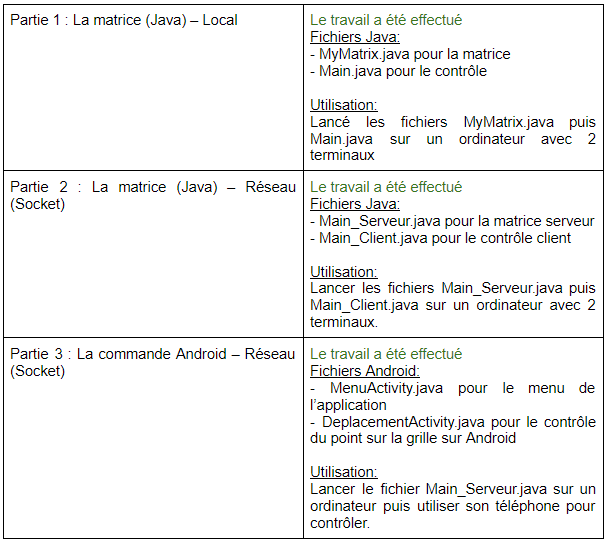
\includegraphics[scale=0.9]{ep1.png}
				\label{ep1}
			\end{figure}
		
		\subsection{Épisode 2}
			\paragraph*{}
			
			\begin{figure}[H]
				\centering
					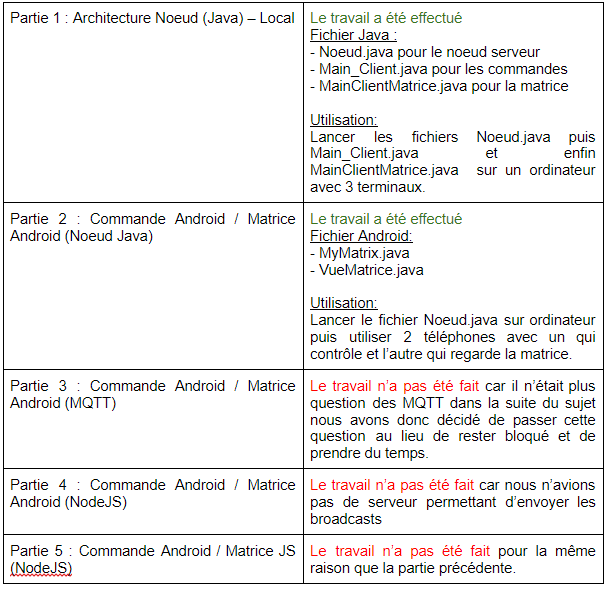
\includegraphics[scale=1]{ep2.png}
				\label{ep1}
			\end{figure}
		
		\subsection{Épisode 3}
			\paragraph*{}
			
			\begin{figure}[H]
				\centering
					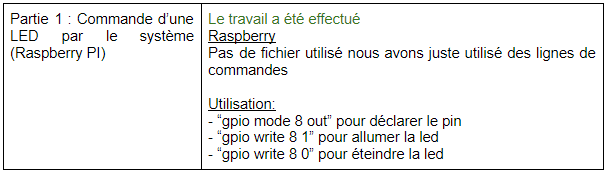
\includegraphics[scale=0.8]{ep3_1.png}
				\label{ep1}
			\end{figure}
			
			\begin{figure}[H]
				\centering
					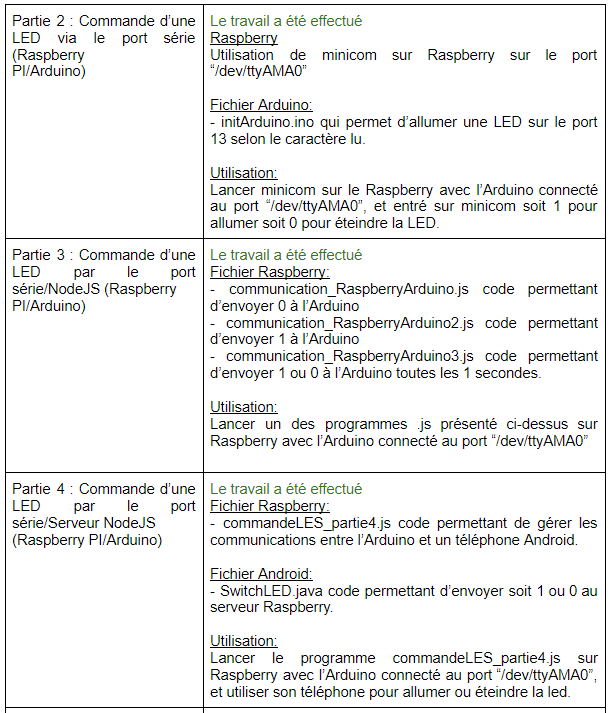
\includegraphics[scale=0.8]{ep3_2.png}
				\label{ep1}
			\end{figure}
			
			\begin{figure}[H]
				\centering
					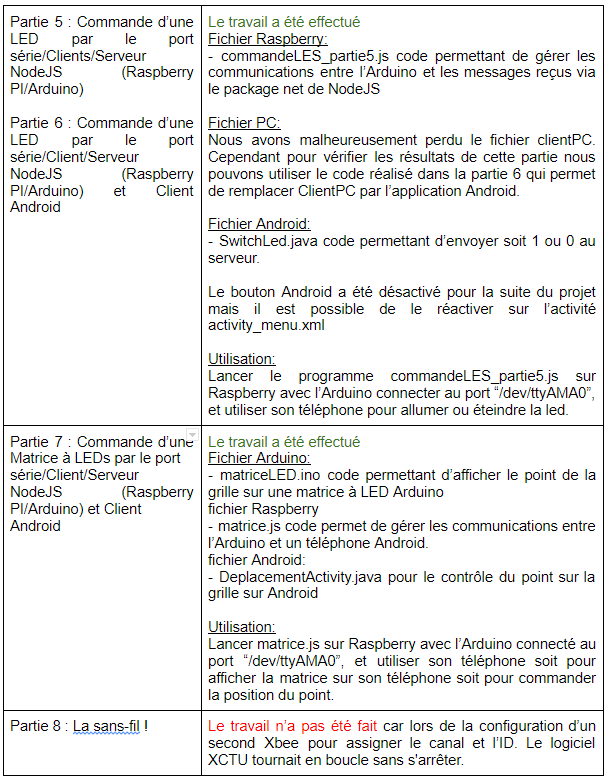
\includegraphics[scale=1]{ep3_3.png}
				\label{ep1}
			\end{figure}
		
		
		\subsection{Épisode 4}
			\paragraph*{}
			
			\begin{figure}[H]
				\centering
					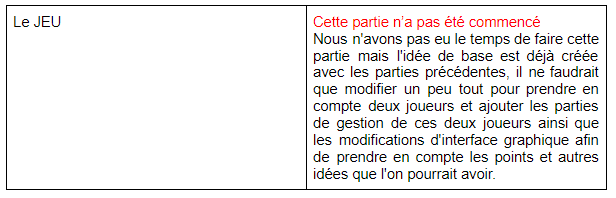
\includegraphics[scale=1]{ep4.png}
				\label{ep1}
			\end{figure}
		
		
		\subsection{Autres implémentations faites}
			\paragraph*{}
			Nous avons ajouté certaines fonctionnalités supplémentaires qui ont surtout servi à une meilleure ergonomie de l'application.
			
			Nous pouvons cité par exemple la traduction complète de l'application en Anglais (US) et Français avec une possibilité d'ajout d'autres langues si nécessaire.
			
			Nous avons également ajouté des messages s'affichant en bas de l'écran en cas de connexion bien réalisé ou mal réalisée et pareil pour la déconnexion.
			
			Nous avons ajouté une activité de paramètres qui devait servir au départ à inscrire dans une box l'IP du serveur et les ports à utiliser mais nous n'avons pas eu le temps de finir cette partie qui est pourtant très proche de la fin !
			
			Enfin, afin de mieux nous organiser dans notre travail, nous avons utilisé GitHub afin de travailler à plusieurs et à distance et également pour versionner le projet pour éviter des problèmes qui aurait pu survenir en cas d'écrasement d'un fichier fonctionnel et par la perte de son contenu. Pour utiliser GitHub nous avons utilisé le logiciel sur Windows GitKraken (https://www.gitkraken.com/).
	
	\section{Conclusion}
		\paragraph*{}
		Nous n'avons pas réussi à tout implémenter notamment dû aux conditions sanitaires actuelles et également à certains problèmes tel le XBEE qui ne se connectait pas. Malgré cela, une très grosse partie du projet a été réalisé avec le détail des codes dans les différents sous-dossiers présents dans le dossier principal. Nous avons travaillé le côté fonctionnel mais aussi un peu le côté ergonomique en ajoutant des petites fonctionnalités bonus tel la traduction complète de l'application ou les ajouts des messages si la connexion s'est bien faite ou si la déconnexion s'est bien passée. Vous pouvez voir le résultat de l'application dans le dossier ou alors sinon dans la section Annexes qui suit il y a quelques screenshots de l'application sur un téléphone Samsung A40.
	
	\section{Annexes}
		\paragraph*{}
		Je met des screenshots de l'application Android avec quelques fonctionnalités actives au cas où elles ne fonctionneraient pas sur un autre appareil.
		
		\begin{figure}[H]
			\centering
				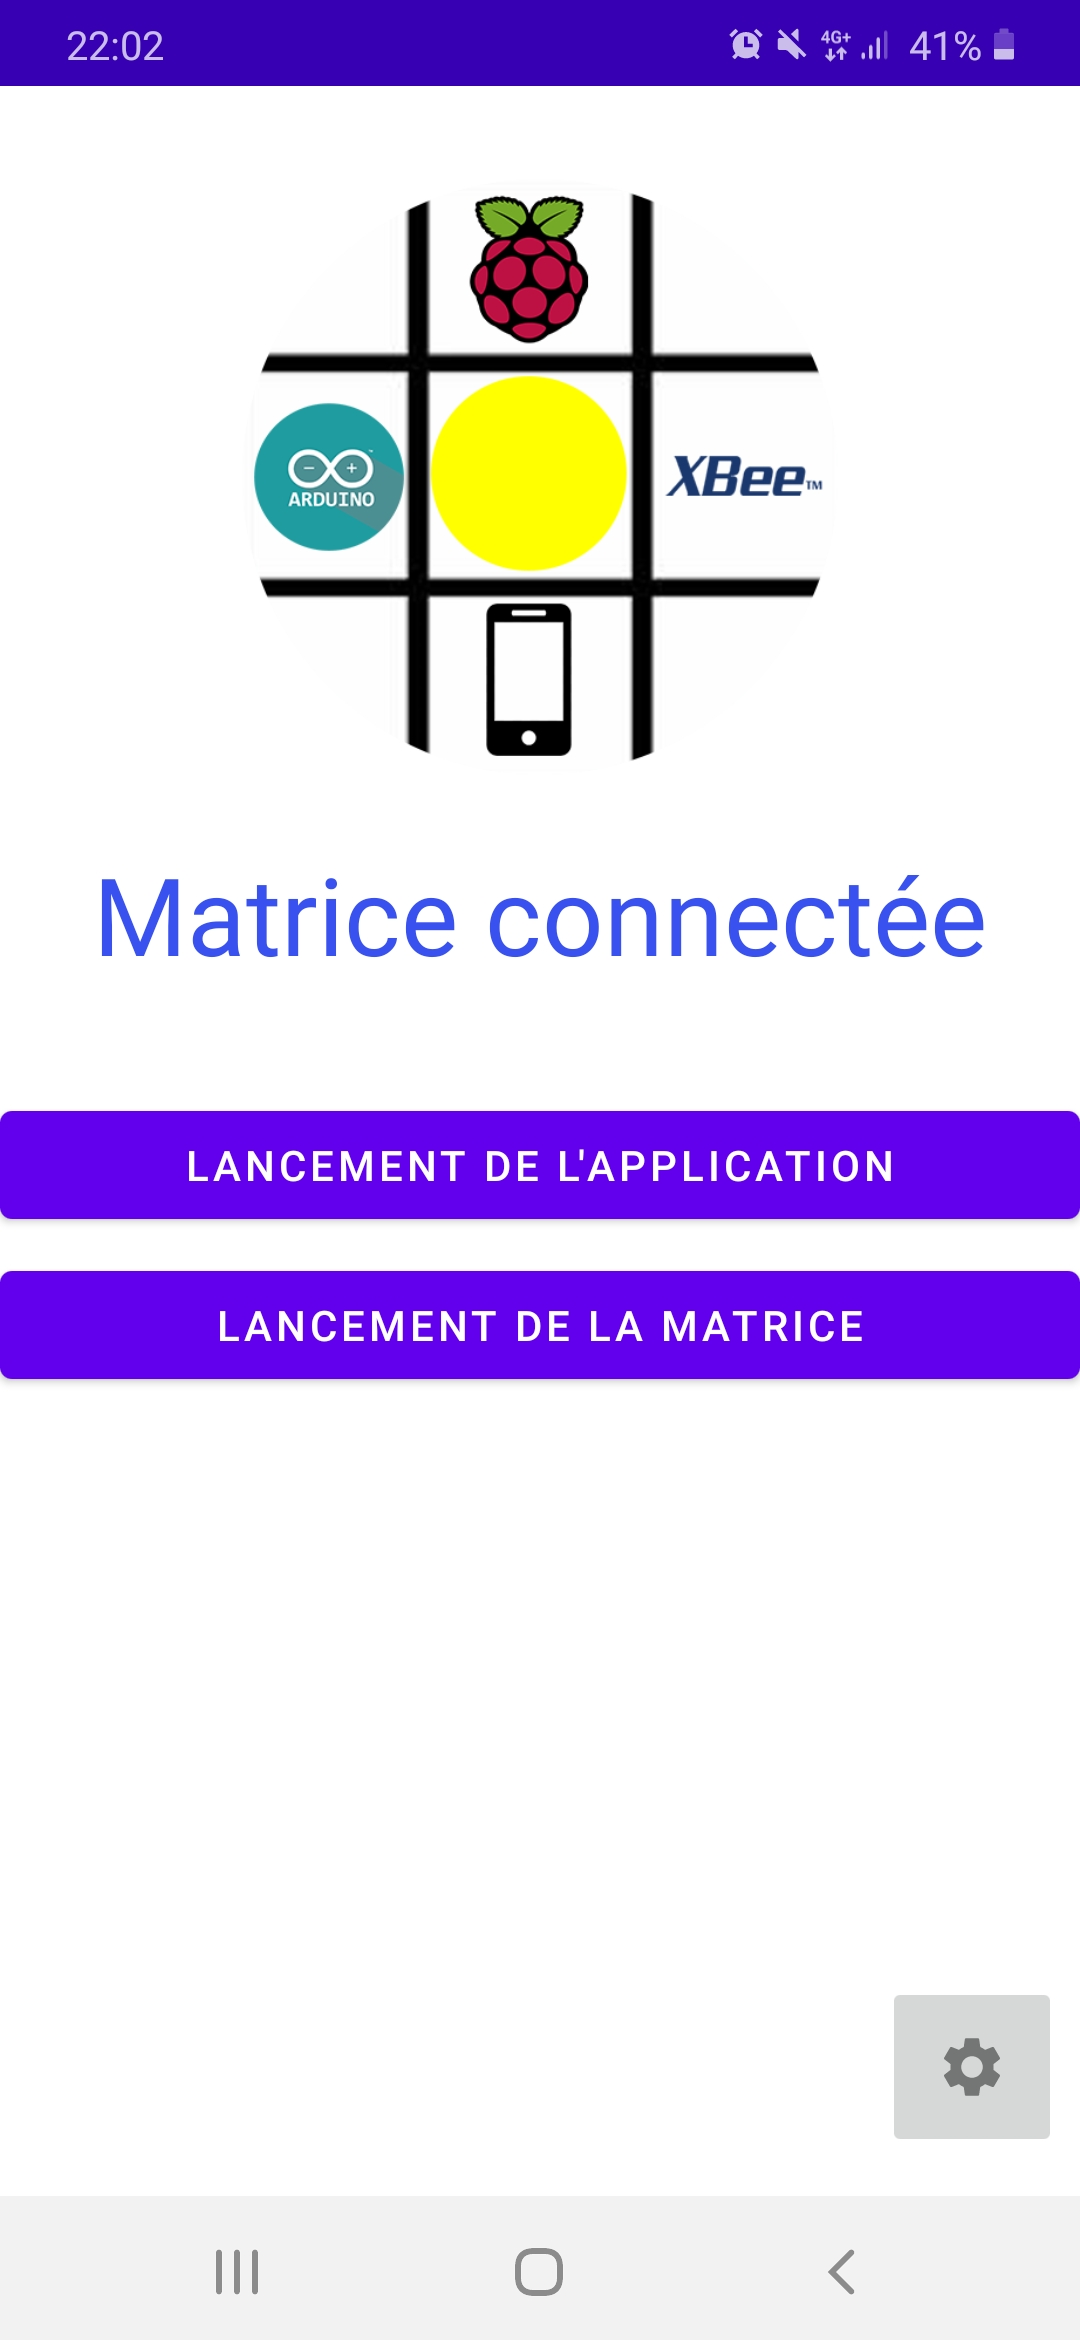
\includegraphics[scale=0.14]{menu.jpg}
				\caption{Menu principal de l'application}
		\end{figure}
		
		\begin{figure}[H]
			\centering
				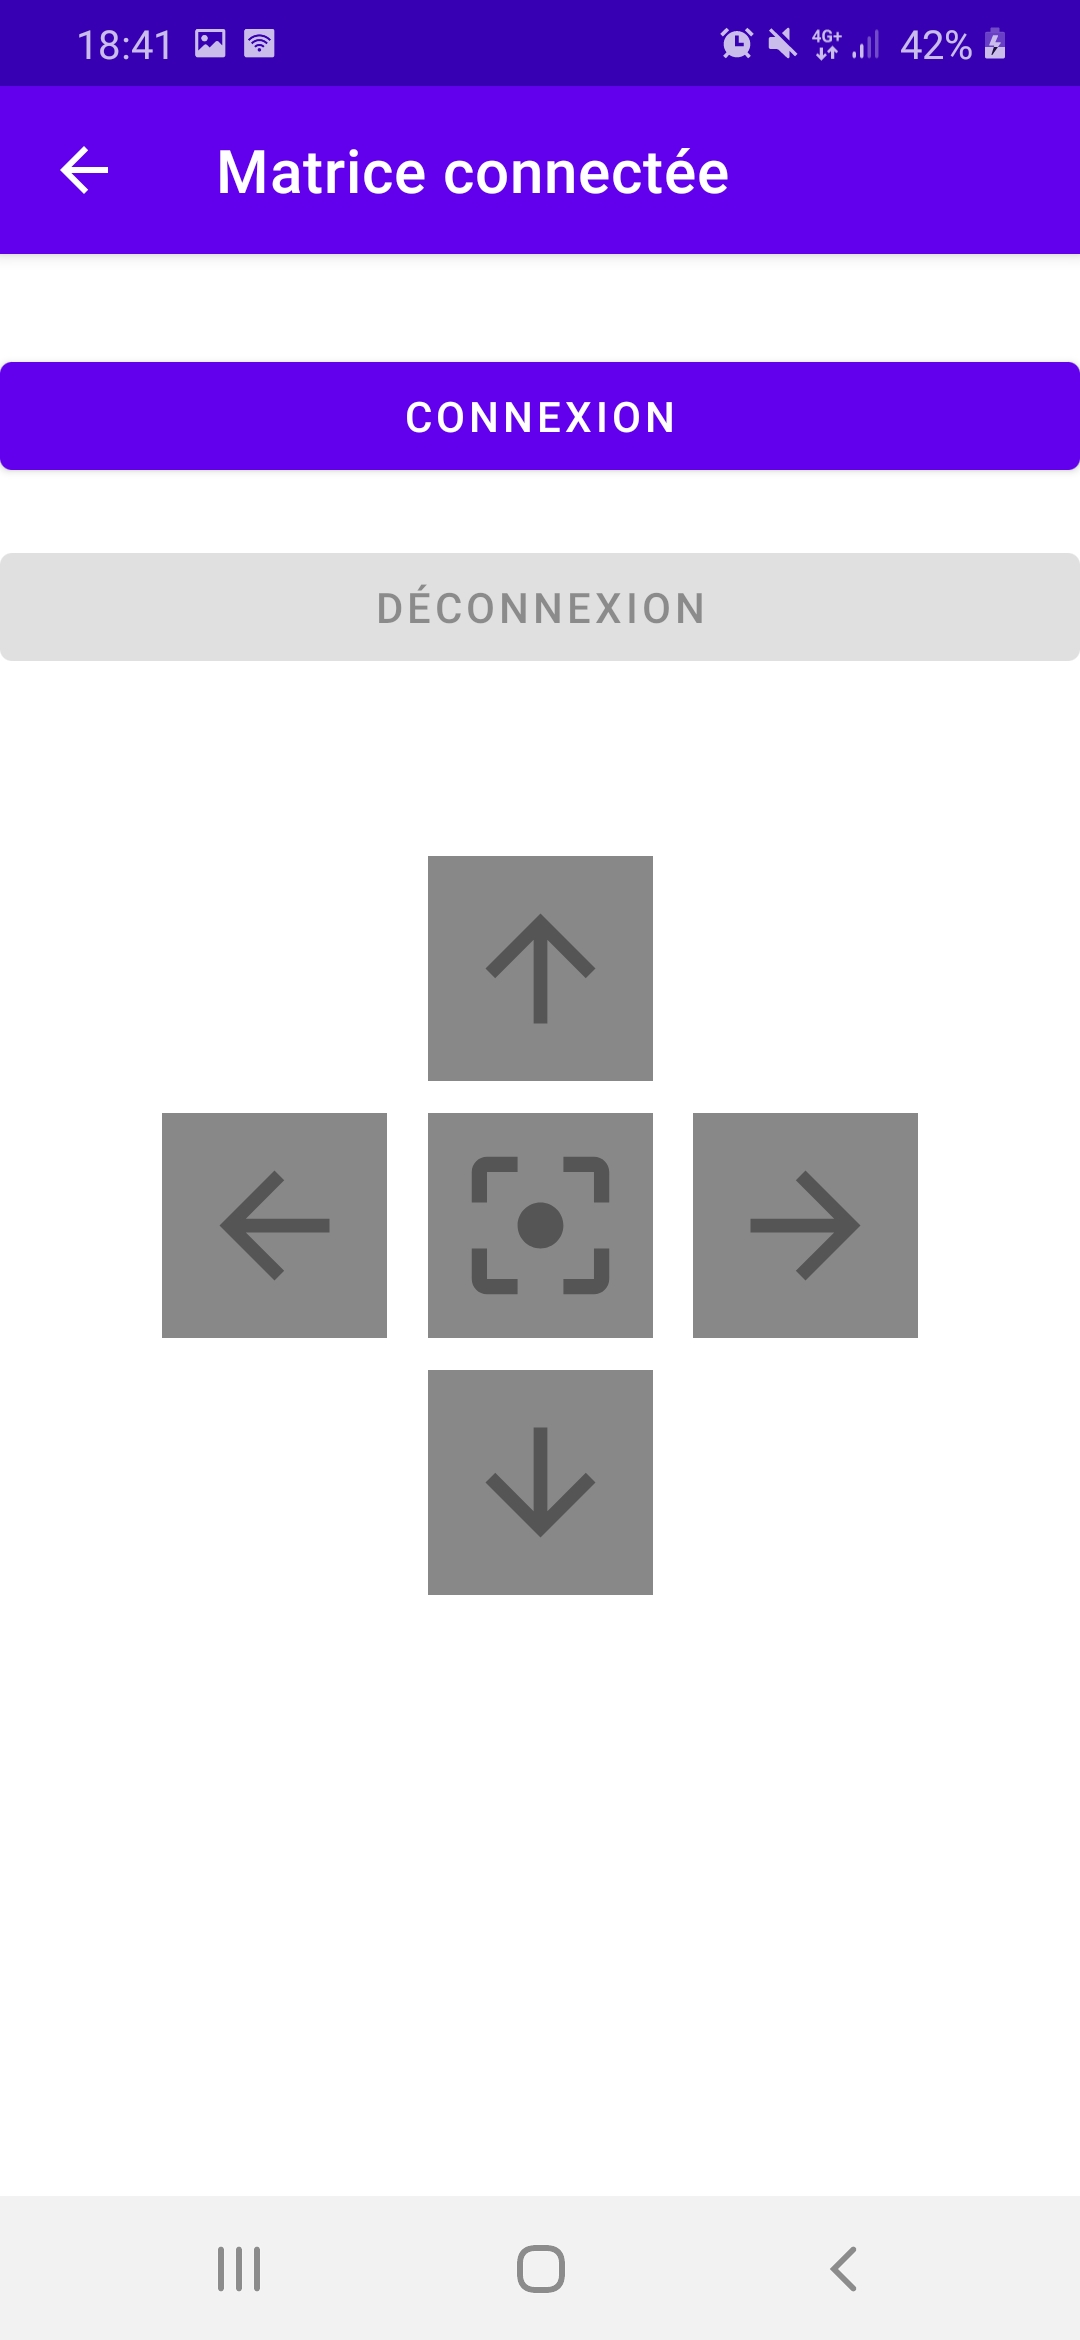
\includegraphics[scale=0.2]{depnco.jpg}
				\caption{Activité déplacement du point en non connecté}
		\end{figure}
		
		\begin{figure}[H]
			\centering
				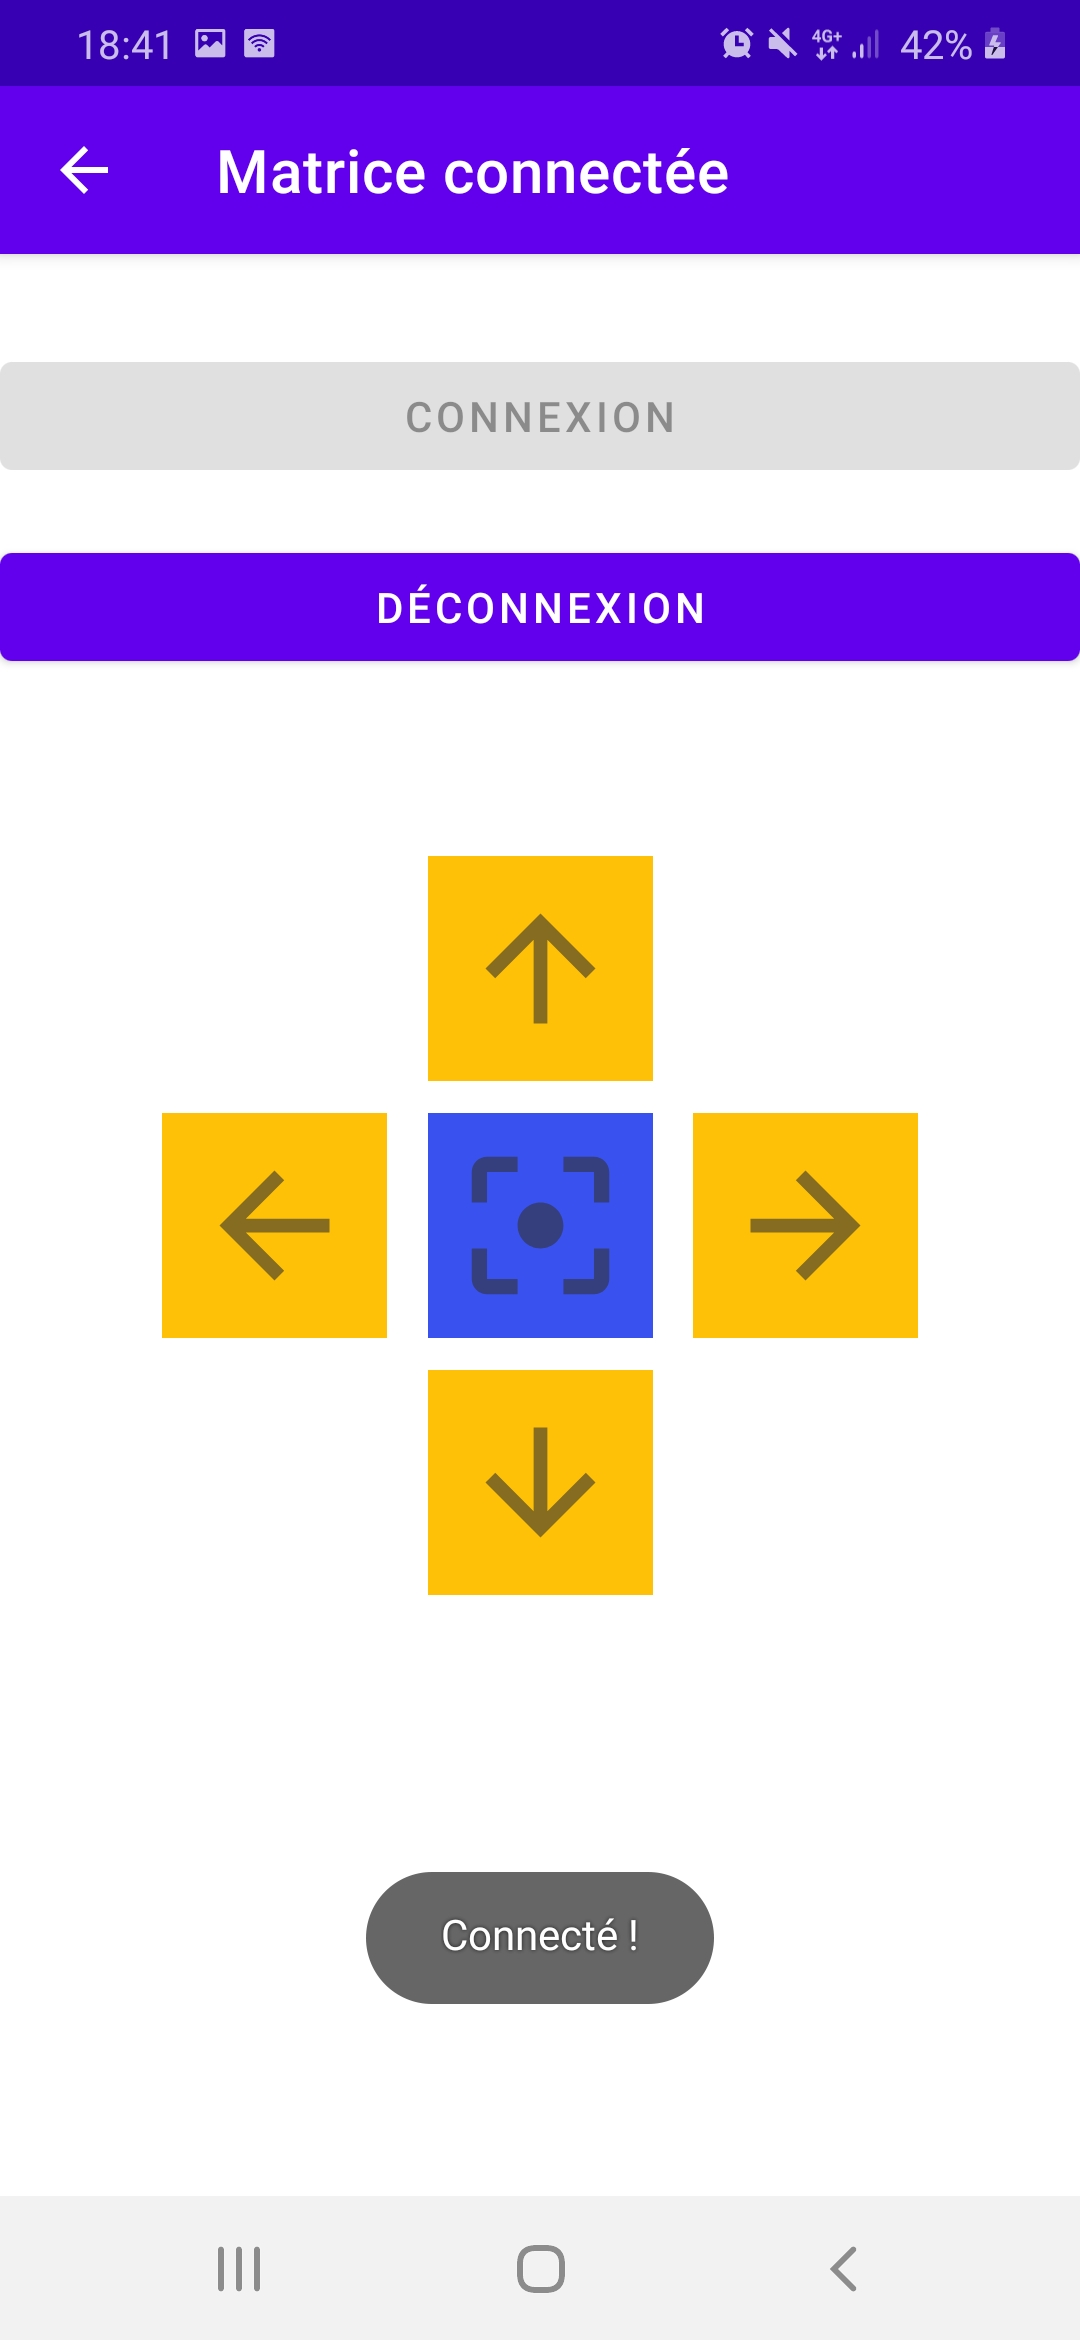
\includegraphics[scale=0.2]{depco.jpg}
				\caption{Activité déplacement du point en connecté}
		\end{figure}
		
		\begin{figure}[H]
			\centering
				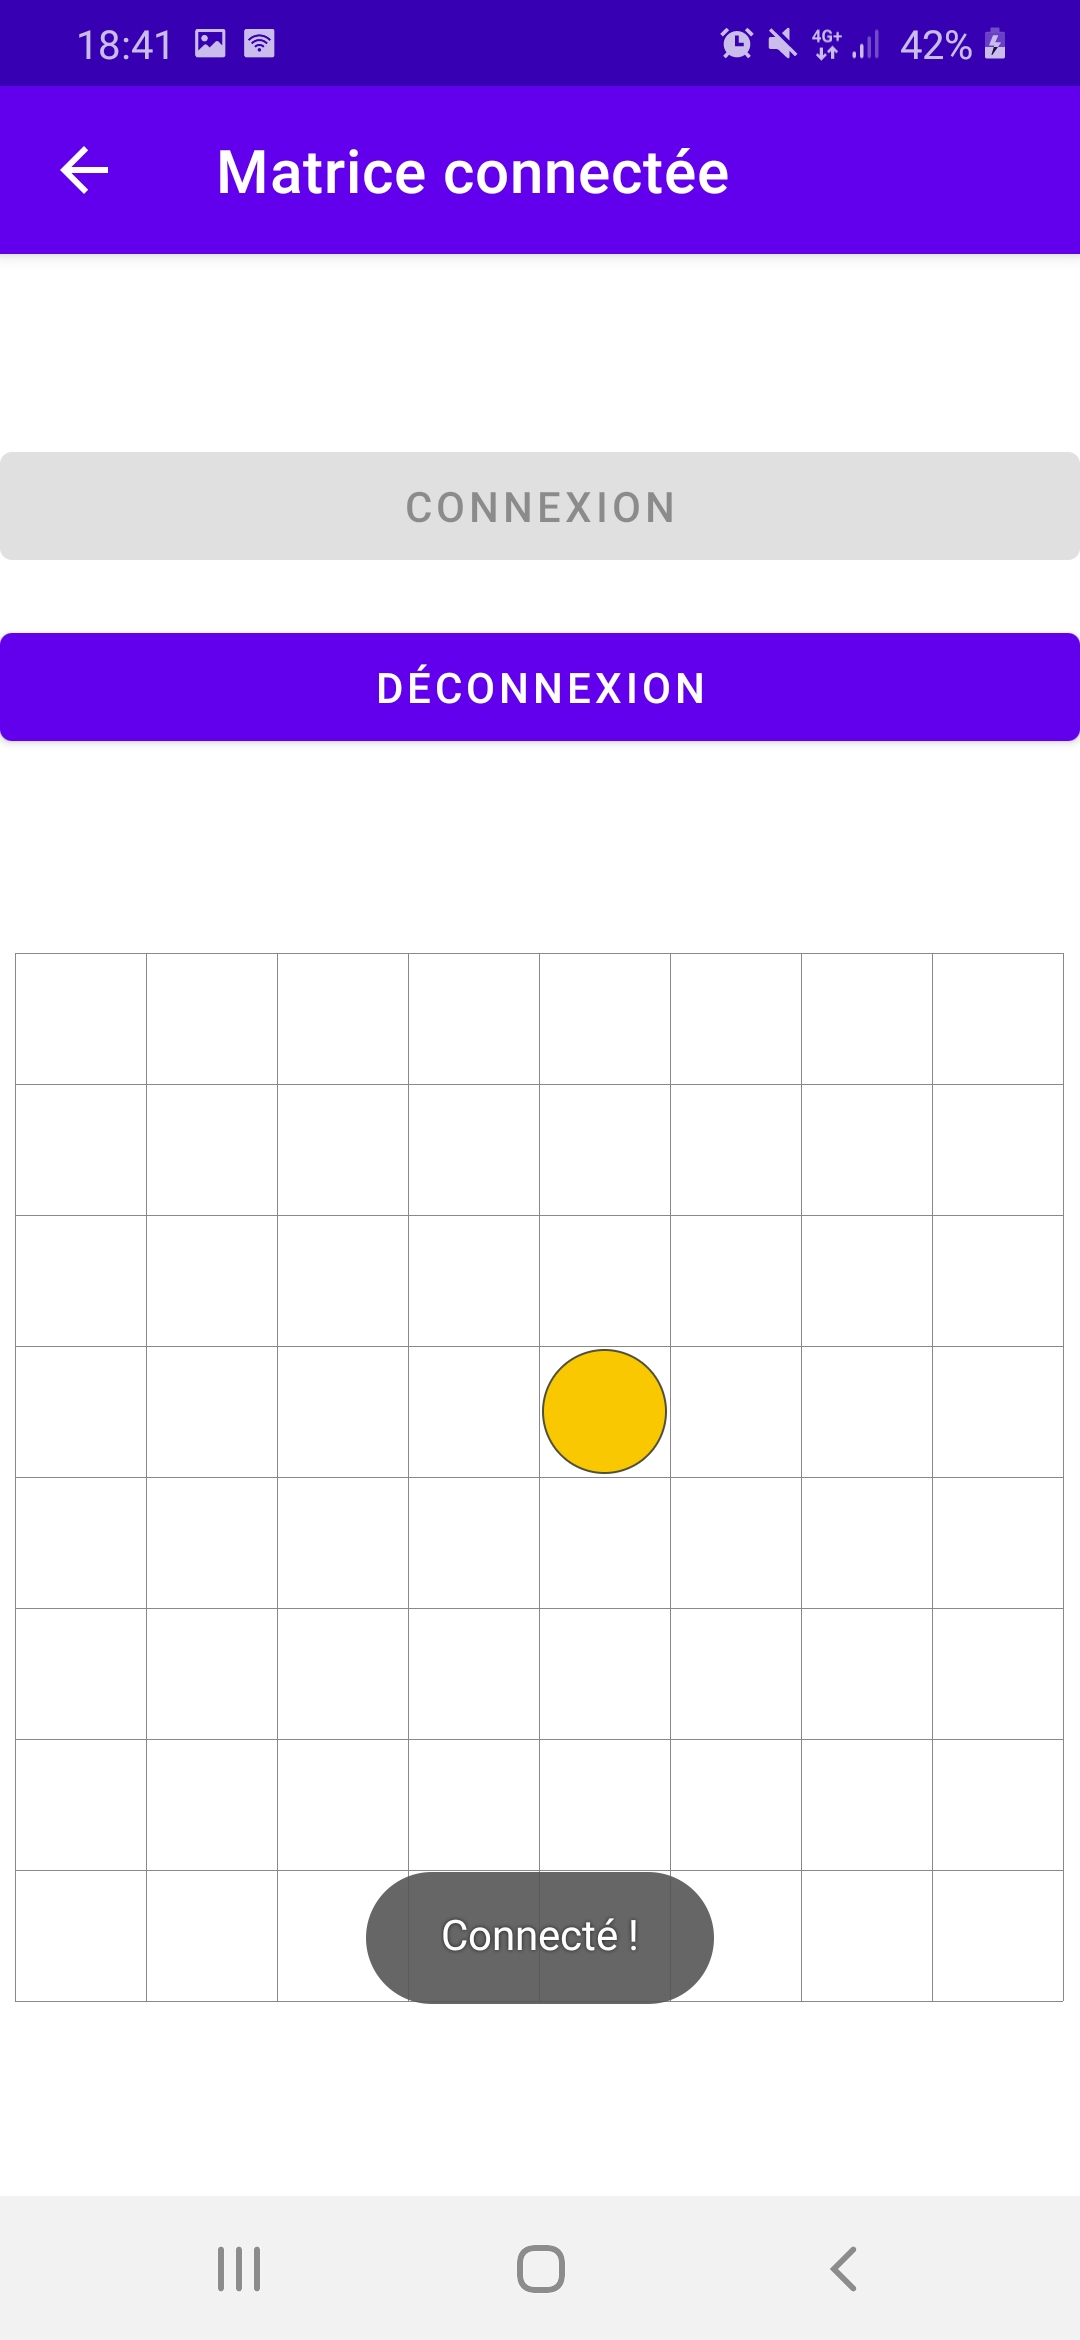
\includegraphics[scale=0.2]{matco.jpg}
				\caption{Activité affichage de la matrice en connecté}
		\end{figure}
		
		\begin{figure}[H]
			\centering
				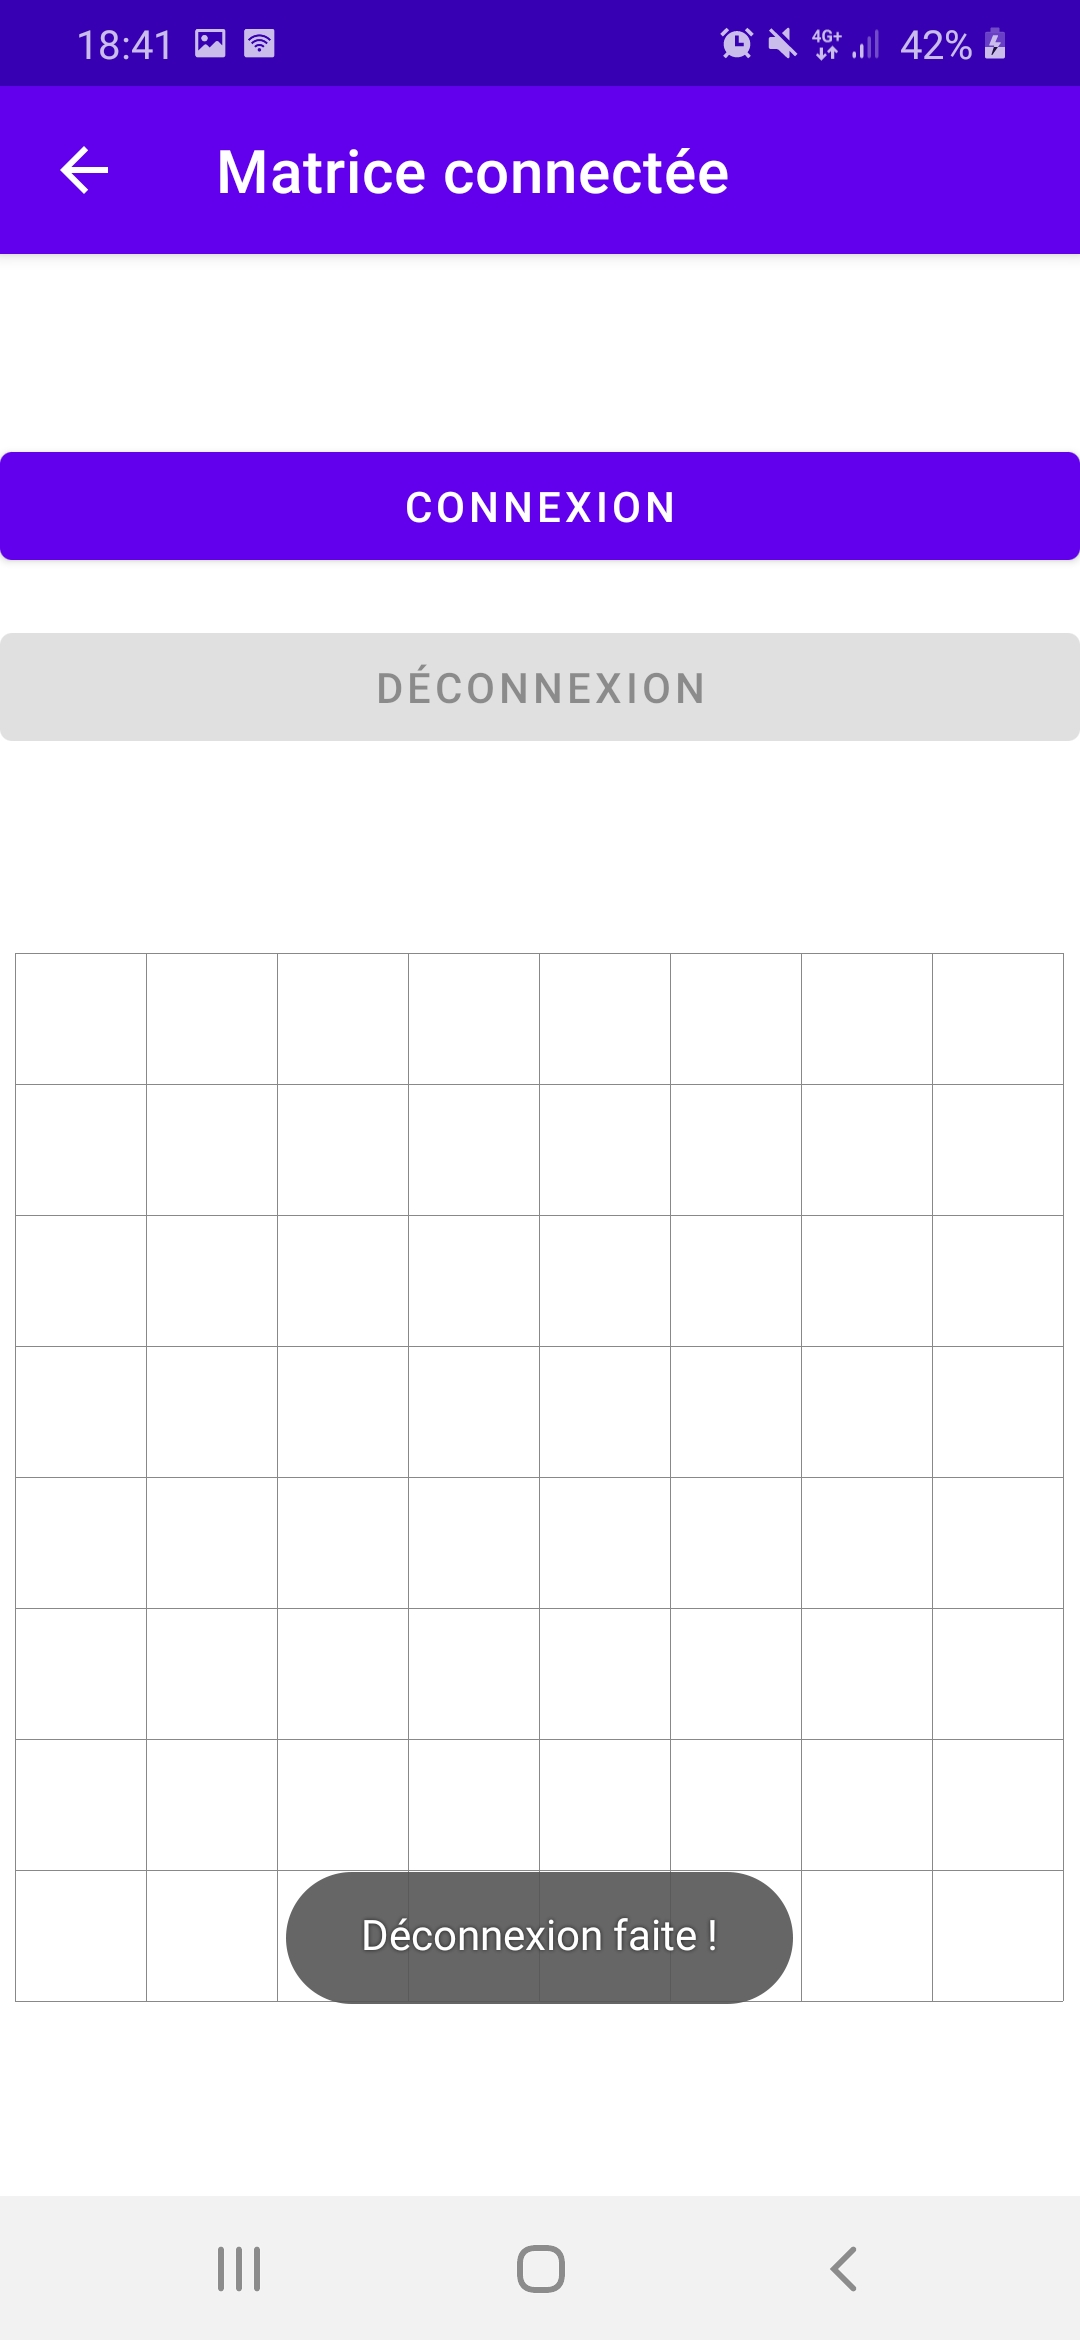
\includegraphics[scale=0.2]{matnco.jpg}
				\caption{Activité affichage de la matrice en non connecté}
		\end{figure}
		
		\begin{figure}[H]
			\centering
				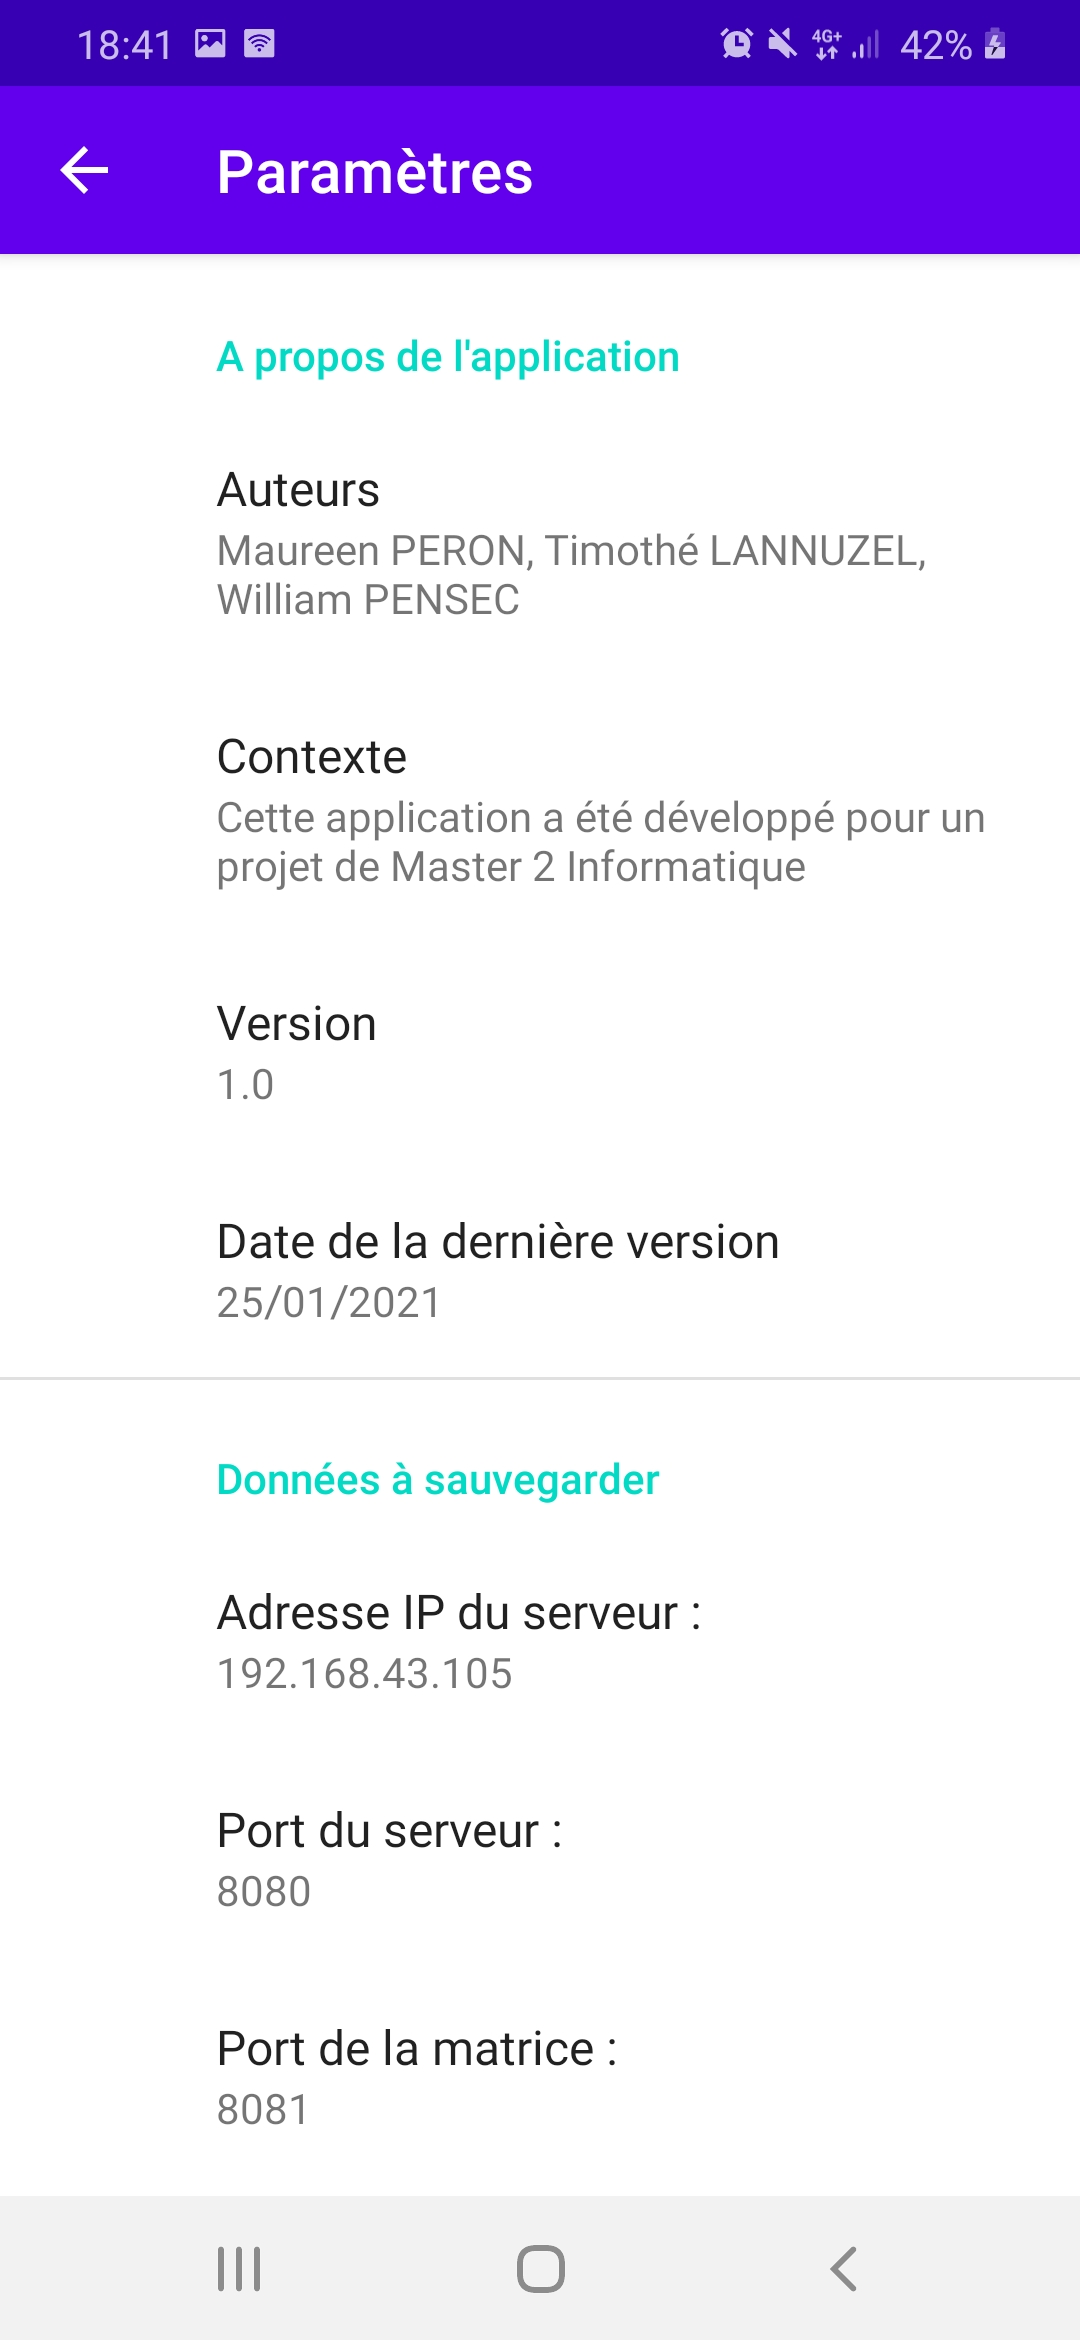
\includegraphics[scale=0.2]{param.jpg}
				\caption{Activité paramètres}
		\end{figure}

	\clearpage
\end{document}